\chapter{Stand van zaken}
\label{ch:stand-van-zaken}

% Tip: Begin elk hoofdstuk met een paragraaf inleiding die beschrijft hoe
% dit hoofdstuk past binnen het geheel van de bachelorproef. Geef in het
% bijzonder aan wat de link is met het vorige en volgende hoofdstuk.

% Pas na deze inleidende paragraaf komt de eerste sectiehoofding.
%
%Dit hoofdstuk bevat je literatuurstudie. De inhoud gaat verder op de inleiding, maar zal het onderwerp van de bachelorproef *diepgaand* uitspitten. De bedoeling is dat de lezer na lezing van dit hoofdstuk helemaal op de hoogte is van de huidige stand van zaken (state-of-the-art) in het onderzoeksdomein. Iemand die niet vertrouwd is met het onderwerp, weet er nu voldoende om de rest van het verhaal te kunnen volgen, zonder dat die er nog andere informatie moet over opzoeken \autocite{Pollefliet2011}.
%
%Je verwijst bij elke bewering die je doet, vakterm die je introduceert, enz. naar je bronnen. In \LaTeX{} kan dat met het commando \texttt{$\backslash${textcite\{\}}} of \texttt{$\backslash${autocite\{\}}}. Als argument van het commando geef je de ``sleutel'' van een ``record'' in een bibliografische databank in het Bib\TeX{}-formaat (een tekstbestand). Als je expliciet naar de auteur verwijst in de zin, gebruik je \texttt{$\backslash${}textcite\{\}}.
%Soms wil je de auteur niet expliciet vernoemen, dan gebruik je \texttt{$\backslash${}autocite\{\}}. In de volgende paragraaf een voorbeeld van elk.
%
%\textcite{Knuth1998} schreef een van de standaardwerken over sorteer- en zoekalgoritmen. Experten zijn het erover eens dat cloud computing een interessante opportuniteit vormen, zowel voor gebruikers als voor dienstverleners op vlak van informatietechnologie~\autocite{Creeger2009}.

%	EFFECTIEVE LITERATUURSTUDIE

Dit hoofdstuk bestaat uit een zeer uitgebreide literatuurstudie, waarin de kern van het probleem wordt opgesplitst in verschillende delen. In het eerste deel wordt er uitleg gegeven over JavaScript zelf en diens evolutie. Vervolgens volgt er een groot deel over de frameworks Node.js en Express, erna bekijken we het belang van testen en monitoren van software en breiden we uit naar een analyse van zulke monitoringssoftware. In het tweede deel wordt er onderzoek gedaan naar de vraag van Kayzr. Wat wordt er verwacht, welk inzicht moet er gegeven worden, welke features moeten worden uitgewerkt. 

\section{Javascript}
\label{sec:javascript}
Javascript is een programmeertaal gemaakt voor het web, waarmee statische websites kunnen omgezet worden naar dynamische en interactieve websites. Doordat het een enorm krachtige scripttaal is dat speciaal werd ontwikkeld om de functionaliteiten van een doorsnee HTML/CSS-pagina uit te breiden, wordt het bijna onmogelijk om nog iets in te beelden dat niet geïmplementeerd kan worden m.b.v. Javascript. De taal is weakly-typed, functioneel, event-driven en dynamisch. JavaScript bevat een bibliotheek van standaardobjecten samen met specifieke taalelementen zoals operatoren, controlestructuren, enz... Deze kern of 'core' kan makkelijk uitgebreid worden met extra objecten waardoor men JavaScript makkelijk kan specifieren als \textit{Client-side JavaScript} en \textit{Server-side JavaScript}. Client-side JavaScript wordt bijvoorbeeld gebruikt om interactie met de gebruiker te verzorgen zoals muiskliks, keyboard-hits en nog veel meer. Server-side JavaScript houdt zich eerder bezig met het achterliggende van een site, bijvoorbeeld om een webapplicatie te doen communiceren met een databank. Een zeer bekende en veel gebruikte Server-side JavaScript variant is Node.js, waarover later meer uitleg wordt gegeven. \autocite{Javascript2019}

\subsection{Tijdlijn van JavaScript}
\label{sec:jsTimeline}

Javascript heeft echter een hele evolutie achter de rug. Ontstaan in mei 1995, wordt de taal na vele updates nog steeds dagdagelijks gebruikt en kan het wereldwijde web niet meer ingebeeld worden zonder. Brendan Eich, de auteur van de taal, werkte in 1995 samen met Netscape Communications, de makers van de eerste grote webbrowser genaamd Netscape Navigator, om een taal te implementeren in hun browser waar webontwikkelaars gebruik van zouden kunnen maken. Java, een zeer zware programmeertaal met tal van functionaliteiten was de eerste keuze van Netscape, maar Eich schreef uiteindelijk zijn eigen idee uit van een scripttaal in nog geen 10 dagen en overtuigde Netscape om de lichte, schaalbare en Java-complementerende-taal te adopteren \autocite{Rangpariya2019}. Javascript, toen onder de naam Mocha en vervolgens LiveScript, was geboren en zette de wereld van webontwikkelaars op zijn kop.

Netscape bracht nieuwere versies van JavaScript uit, maar Microsoft dreigde die te onttronen. Niet zoveel later, bracht Microsoft Internet Explorer 3 uit met een eigen variant op Javascript, namelijk JScript. Dit was een zware slag voor Netscape, aangezien Microsoft hen hierdoor zou voorbijsteken, maar was wel een grote stap in de evolutie van JavaScript zoals wij het nu kennen. Dit bracht echter problemen met zich mee, want bedrijven zouden telkens eigen versies van JavaScript uitbrengen wat voor veel compatibiliteitproblemen zou zorgen. Uiteindelijk, in 1997, werd JavaScript 1.1 gestandaardiseerd dankzij het European Computer Manufacturers Association en werd omgedoopt tot ECMAScript. \autocite{Wiley2016} Deze standaard, namelijk ES1 (versie 1), zou dan vertakkingen verhelpen. Implementaties van ECMAScript, waaronder JScript, ActionScript, maar dus ook JavaScript zelf, zouden dan telkens ECMAScript implementeren waardoor de core van de varianten telkens hetzelfde blijft. Nu, in 2019; is JavaScript nog steeds enorm populair en implementeert ondertussen al de 9e versie van ECMAScript: ES2018. Na ES5 is ECMASCRIPT overgeschakeld naar jaarlijkse releases, startend vanaf ES2015.

\subsection{Waarom JavaScript?}
\label{sec:jsWhy}

JavaScript is niets voor niets enorm populair, zelfs nog steeds na al die jaren, dankzij de vele voordelen dat de taal met zich meebrengt. En die lijst van voordelen wordt per iteratie alleen maar groter. Hieronder worden er enkele kernvoordelen opgesomd.

\subsubsection{Dynamisch en weakly-typed}
\label{sec:dynamic}

Een dynamisch getypeerde taal slaat neer op het feit dat het type van waarden kan veranderen tijdens uitvoertijd. Dit betekent bijvoorbeeld dat een variabele string plots kan gebruikt worden om een som te maken met een getal. Dit maakt uitvoertijd en compileertijd aanzienlijk sneller doordat er niet voortdurend controles moeten plaatsvinden. Dit zorgt voor hoge performantie, maar slechte nauwkeurigheid.

\subsubsection{DOM-manipulatie}
\label{sec:DOM}
\begin{figure}
	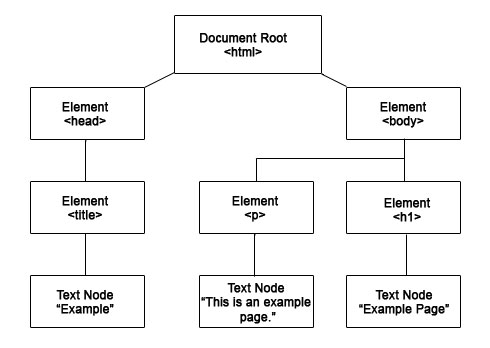
\includegraphics[width=\linewidth]{dom.jpg}
	\caption{Voorbeeld van een DOM structuur.}
	\label{fig:dom}
\end{figure}

De DOM, ofwel Document Object Model, is kortweg het skelet van een HTML-pagina. De structuur van het skelet beschrijft een boomstructuur, waardoor een element een ouder, broer, kind, kleinkind, achterkleinkind, enz... van een element kan zijn. Het HTML element is de wortel van de boom. Client-side JavaScript wordt grotendeels gebruikt om deze boomstructuur te manipuleren. Hierdoor kunnen we HTML elementen toevoegen, verwijderen, stijlen manipuleren, enz... allemaal tijdens uitvoertijd. \textcite{Kantor2017}

\subsubsection{Prototype-based}
\label{sec:prototypeBased}

In JavaScript kan een object eigenlijk aanzien worden als een Array. Hierdoor kunnen ze heel gemakkelijk aan de eigenschappen van een object aan en kunnen we deze ook makkelijk tijdens uitvoertijd aanpassen. Ook kunnen we op deze manier makkelijk eigenschappen aan bestaande objecten toevoegen. In JavaScript wordt gebruikt van de 'dot-notatie' of van de 'haakjesnotatie'. 

	\begin{verbatim}
	foo.bar = 10;
	foo['bar'] = 10;
	const bar = foo.bar;
	foo['bar2'] = bar;
	\end{verbatim}

\subsubsection{Event-driven}
\label{sec:eventDriven}

JavaScript is event-driven, wat betekent dat de code vooral kijkt naar acties van de gebruiker. Bijvoorbeeld: Wanneer een gebruiker op een knop klikt, wil je dat met een animatie de knop heeen en weer beweegt, tekst op je scherm verschijnt, en een server-request wordt gestuurd. 

\subsubsection{Functioneel}
\label{sec:functional}

Sinds ES2015 is JavaScript niet enkel en alleen een object-georiënteerde taal, maar ook een functionele taal. JavaScript was zeer snel met het introduceren van functioneel programmeren (waaronder de populaire arrow-functions). Dit vergemakkelijkte de taal aanzienlijker, aangezien veel minder code geschreven moest worden om hetzelfde resultaat te bereiken.

\subsubsection{Universeel}
\label{sec:universal}

JavaScript wordt sinds ES5 ondersteund door alle moderne browsers! Of er nu in Chrome, Firefox, Safari, Edge of het oude Internet Explorer\footnote{Internet Explorer wordt niet meer verder ontwikkelt, dus ondersteunt het enkel ES2015.} wordt gesurft, ze ondersteunen allemaal JavaScript. D.m.v. de console in de browser te openen kan er al geprogrammeerd worden.





\section{Node.js}
\label{sec:nodeJs}

Node.js is een open-source JavaScript runtime omgeving dat wordt gebruikt voor Server-side toepassingen. Node.js maakt het mogelijk, (of eerder \textit{makkelijker}), om JavaScript nu ook te gebruiken buiten websites maken. Aangezien JavaScript zo'n krachtige taal is, hadden de ontwikkelaars van Node.js een ding in gedachten: JavaScript niet enkel voor browsers, maar ook voor alleenstaande applicatie. Sindsdien evenaart JavaScript aan andere scripttalen, zoals Python. \textcite{Patel2018}

\subsection{Tijdlijn van Node.js}
\label{sec:nodeTimeline}
Node.js' verhaal start in 2009, toen een ontwikkelaar genaamd Ryan Dahl het niet zo goed stelde met Apache Http Servers. 

Zoals beschreven in \autocite{Chaniotis2015}, was (en is in grote mate nog steeds) Apache HTTP, in combinatie met PHP, jarenlang de go-to-taal om webapplicaties te laten communiceren met databases en server-side functionaliteiten toe te voegen aan webapplicaties, zoals authenticatie, file-en-ftpservers, logging en nog veel meer. PHP is echter nooit in het achterhoofd ontwikkeld geweest om hedendaagse, complexe webapplicaties te schrijven. Ten tweede was Apache incapabel om te schalen naar meerdere processorkernen, waardoor de performantie enorm daalde. PHP in combinatie met Apache was gewoonweg niet gemaakt voor de volgende generatie webapplicaties. Andere struikelblokken zijn cross-platform mobiele applicaties en real-time communicatie.

Meer en meer applicaties worden gemaakt met cross-platform compatibiliteit in het achterhoofd, aangezien de toestroming van verschillende nieuwe besturingssystemen en apparaten het meer en meer onmogelijk maken om native apps\footnote{Native Apps zijn applicaties die gemaakt worden met één besturingssysteem in het hoofd. Bv: Android, IOS.} te ontwikkelen. Hierdoor worden bibliotheken en frameworks ontwikkeld zoals React Native, Flutter, Xamarin, Ionic, PhoneGap, enz... die deze nadelen kunnen overbruggen. Deze zijn echter zo krachtig geworden en schenken zoveel nieuwe voordelen, dat server-side talen en frameworks zoals Apache HTTP/PHP eerder een bottleneck vormden. 

Real-time communicatie is nog een factor dat niet ondersteund wordt door Apache. Apache was niet ontwikkeld om berichten te sturen naar de client-side. In de wereld van vandaag, waarin sociale media nog nooit zo'n grote invloed heeft gehad op ons dagelijks leven, is het haast ondenkbaar dat real-time communicatie niet zou kunnen bestaan. 

Dit alles zorgde voor de ontwikkeling van Node.js. Dahl's project werd met open armen ontvangen. Na enkele struikelblokken, kende Node.js in 2011 voor het eerst het licht en wordt nu zo'n tien jaar later, gebruikt in vele moderne applicaties en is nog steeds één van de meest begeerde vaardigheden van een programmeur. \autocite{Patel2018}

Hoewel Apache en PHP nog steeds overduidelijk op plaats één staan, hebben ze hun populariteit enkel nog te danken aan bedrijven die op verouderde software werken, en hun populariteit bij senior ontwikkelaars. PHP blijft een geliefde taal bij velen, maar in \ref{fig:trend} zien we dat Node.js's populariteit duidelijk die van Apache aan het inhalen is. \autocite{SimilarTech}

\begin{figure}[h]
	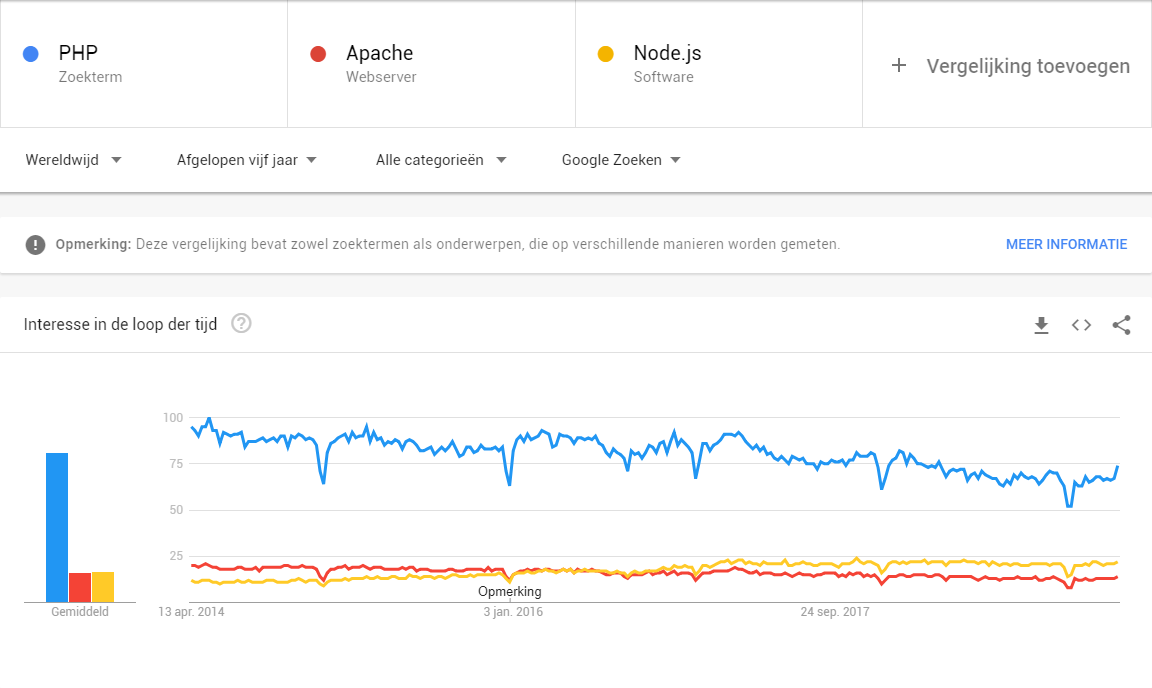
\includegraphics[width=\linewidth]{trend.png}
	\caption{Google searches van PHP (blauw), Apache (rood) en Node.js (geel) in de afgelopen 5 jaar.}
	\label{fig:trend}
\end{figure}

\subsection{Waarom Node.js?}
\label{sec:whyNode}
Node.js is reeds een volwassen server-side framework. Youtube, Yahoo, Google, Amazon, Netflix, Ebay, Reddit, LinkedIn, Paypal, Github, Forbes, Walmart, Uber, NASA, Slack,.. zijn slechts enkele van de duizenden websites die overgeschakeld zijn naar Node.js. En dit zijn geen kleine namen.

Illustrator \textcite{Mehmet2016} toont op een illustratieve wijze de voordelen van Node.js aan. LinkedIn kon hun 15 servers reduceren naar slechts 4 en terwijl de verkeerscapaciteit nog eens verdubbelen. Walmart kon al hun Client-side JavaScript processing naar hun servers verplaatsen, en Ebay kon hun verkeerscapaciteit enorm doen verhogen en hun verbruik enorm doen dalen. De voordelen en functionaliteiten worden hieronder nog eens opgesomd zoals aangegeven door \textcite{Chandrayan2017}.

\subsubsection{nieuw}
\label{sec:new}

JavaScript is relatief gezien een nieuwe taal dat voortdurend geüpdatet wordt. In tegenstelling tot traditionele server-talen zoals Python, PHP, enzovoort. Vele dialecten van JavaScript (zoals TypeScript, CoffeeScript, ClojureScript,...) compileren dan gewoonweg in JavaScript waardoor overschakelen zeer simpel wordt. Doordat Node.js ook in JavaScript geschreven is, maakt dit het makkelijker om de client-server-side-brug over te steken als frontend ontwikkelaar of vice versa. \autocite{ExpressMozilla}

\subsubsection{Asynchroon}
\label{sec:async}

Node.js is sterk afhankelijk van asynchrone en continue programmeerstijl. I/O-bewerkingen worden uitgevoerd door middel van oproepen naar asynchrone functies waarbij een callback moet worden doorgegeven om aan te geven hoe de berekening wordt voortgezet zodra de genoemde I/O-bewerking asynchroon is voltooid. Het Node.js executiemodel bestaat uit een hoofdgebeurtenislus die wordt uitgevoerd op een single-threaded proces. Met behulp van deze \textit{event loop} moet een Node.js server nooit wachten op antwoord, het kan gewoon blijven doordraaien na een oproep van een API Call en kan dankzij een notificatiesysteem op een later moment het antwoord terugsturen. Dit maakt Node.js enorm schaalbaar, in tegenstelling tot Apache dat slechts een gelimiteerd aantal threads kan starten om handelingen uit te voeren.

Het is daarom niet altijd makkelijk om deze soort frameworks te debuggen, en het wordt uiteindelijk een uitdagende taak. Gelukkig zijn hiervoor dan ook weer verschillende hulpmiddelen en tools uitgebracht om dit te vereenvoudigen. Zoals vermeld in ~\autocite{Runtime2017}, kan asynchrone code subtiele bugs opleveren die niet meteen zichtbaar zijn. Hier is nog niet echt onderzoek over gedaan. Waar er honderden vergelijkende studies bestaan over de frameworks zelf en of Node.js een goede optie is, zijn er geen of amper studies over de beste manier om dit te debuggen en hoe men dit het best aanpakt. ~\autocite{Runtime2017} vertelt ons meer over het identificeren van schaalbaarheidsproblemen en het aanrijken van mogelijke oplossingen. Ze maken gebruik van parametrische uitdrukkingen voor runtime monitoring van Node.js toepassingen, maar ze geven toe dat dit nog maar de eerste stap is en dat hier nog meer onderzoek naar kan gedaan worden. Hier wordt later in dit onderzoek dieper op ingegaan.

\subsubsection{Performant}
\label{sec:fast}

Google Chrome's JavaScript engine, V8, is bijzonder snel. Dahl heeft dit verder ontwikkeld voor Node.js en dit maakt het framework enorm performant en efficiënt in het compileren en uitvoeren van code. Veel sneller dan Python, Ruby of Perl.

\subsubsection{npm}
\label{sec:npm}

Node.js kent een enorm bloeiende community. Deel van Node.js is zijn Node Package Manager, ofwel npm, en komt meegeleverd bij de installatie. Via npm kan men uit honderdduizenden pakketjes kiezen voor een JavaScript/Node project makkelijk uit te breiden met extra functionaliteiten in één oogwenk. Dagelijks worden er nieuwe pakketjes toegevoegd aan de packet manager, en is makkelijk één van de redenen waarom Node.js zo populair is, aangezien het ontwikkelen van een webapplicatie enorm vereenvoudigd wordt.   

\section{Express}
\label{sec:express}

\subsection{Waarom Express?}
\label{sec:whyExpress}

\textcite{ExpressMozilla} vertelt ons dat echter niet alles rechtstreeks door Node.js wordt ondersteund. Als men bijvoorbeeld routing aan een webapplicatie wenst toe te voegen, zoals HTTP \textsl{GET, POST, PUT, DELETE,} enzovoort... of URL-paden met specifieke requests, statische bestanden weergeven... moet men die code zelf schrijven. Herinner echter het npm-systeem van Node.js. Eén van die honderdduizenden pakketjes is namelijk Express, en is makkelijk \textit{het} populairste Node framework en is zelfs de grondlegger van duizenden andere pakketjes. Express wordt om deze reden door bedrijven dan ook vaak in combinatie gebruikt met Node.js, waaronder Kayzr. 

\subsubsection{Request Handlers}
\label{sec:reqHandlers}

Dankzij Express wordt het zeer gemakkelijk om routering in je applicatie toe te voegen. Indien een GET request gemaakt wordt in de frontend naar een bepaalde URL, is dit zeer gemakkelijk om op te vangen m.b.v. Express. Voor elke soort request en URL kan Express logica uitvoeren en code makkelijk verder delegeren.

\subsubsection{Views}
\label{sec:expressViews}

Express kan statische bestanden zoals HTML, CSS en afbeeldingen laten weergeven in de browser dankzij render engines. Makkelijk om bijvoorbeeld foutpagina's te weergeven.

\subsubsection{Modulair}
\label{sec:expressModularity}

Modulariteit is een kerneigenschap van Express. Express is \textit{unopinionated}, wat wil zeggen dat er niet echt een gouden regel is om een doel in Express te bereiken. Doelen kunnen op meerdere manieren bereikt worden, waardoor het makkelijker is voor ontwikkelaars om een bepaalde taak uit te voeren. Dankzij modulariteit kan het framework ook volledig ingesteld worden naar wens, van poorten en routers, het instellen van een databank tot het toevoegen van Express middleware. 

\subsubsection{Middleware}
\label{sec:expressMiddleware}

Wellicht de krachtigste functie van Express is de eigenschap tot het gebruik maken van middleware. Middleware wordt voortdurend gebruikt in Express. Wanneer een request binnenkomt, wordt deze doorgestuurd door nul, één of meerdere middleware die elk iets doen met de request, tot deze uiteindelijk wordt afgehandeld. De volgorde waarin een request de middleware doorloopt, is volledig afhankelijk van de programmeur. Net zoals Node.js, kent Express ook een enorm grote bibliotheek aan middleware die men kan gebruiken in een applicatie en is alsook helemaal verkrijgbaar via npm. Hierdoor kunnen ontwikkelaars zelf hun middleware schrijven, bestaande middleware downloaden en deze inpluggen in hun applicatie. Middleware kan gaan van Http-request loggers tot cookie-parsers en veel meer. De mogelijkheden zijn praktisch oneindig. Foutmeldingen zijn een goed voorbeeld van Express Middleware. Wanneer ergens iets fout gaat, roept Express de Error-Handler op, die dan zelf de request afwerkt. Monitoringstoepassingen in Node.js maken vaak gebruik van middleware. Hierover volgt meer info in het volgende hoofdstuk.

	\begin{lstlisting}[language=JavaScript, breaklines=true,
						numbers=left, frame=single,
						caption={Express code flow voorbeeld.},
						label=code:expressexample]
	var express = require('express');
	var app = express();
	
	// An example middleware function
	var a_middleware_function = function(req, res, next) {
	// ... perform some operations
	// Call next() so Express will call the next middleware function in the chain.
	next();
	}
	
	// Function added with use() for all routes and verbs
	app.use(a_middleware_function);
	
	// Function added with use() for a specific route
	app.use('/someroute', a_middleware_function);
	
	// A middleware function added for a specific HTTP verb and route
	app.get('/', a_middleware_function);
	
	app.listen(3000);
	\end{lstlisting}
	
	
Middleware schrijven is op zich niet moeilijk. Men kan een enkele functie schrijven, of een heel takenpakket, die men dan als het ware injecteert in een request afhandeling. In een middleware functie verkrijgt men dan een req object, dat van de router kan komen of van een andere middleware, waar dan iets mee kan gedaan worden. Wanneer alles is uitgevoerd, roept de middleware de next-functie op, die dan het nieuwe res, of result, object doorstuurt naar de volgende middleware. Het kan ook zijn dat de middleware de next-functie niet oproept, wat betekent dat dit de laatste stop was van router. 

\begin{figure}[h]
	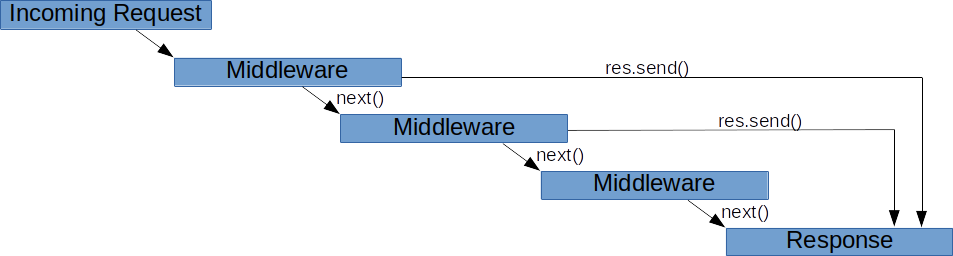
\includegraphics[width=\linewidth]{middleware.png}
	\caption{Schema van de werking van middleware, gebruikt van \cite{middleware}}
	\label{fig:middleware}
\end{figure}

\section{Testen en Monitoring}
\label{sec:testAndMonitoring}

Testen schrijven. Of men nu alleen aan software werkt, of in team in een bedrijf, elke programmeur met een gezond verstand zal kunnen vertellen over het belang van testen schrijven. Iets waar vaak wordt tegenop gekeken, maar het is nodig voor een een geslaagd werkend product op te leveren. Meer en meer bedrijven gaan dit dan ook verplichten in hun implementatieproces. 

Testen en monitoring zijn twee termen dat dicht bij elkaar horen. Bijna elke programmeur kent dan ook het belang van testen schrijven. D.m.v. testen te implementeren kan men kwaliteitsvoller code schrijven, fouten sneller opsporen en is de software een pak robuuster. Het toevoegen van nieuwe functionaliteiten kan code niet meer breken en daardoor kan software langer meegaan. 

\subsection{Agile Testing}
\label{sec:agile}

Agile testing is een methodologie, ontstaan rond 1990, waarin software incrementeel en iteratief wordt uitgewerkt en dat op de dag van vandaag in vele bedrijven wordt gehanteerd. Vooraleer er effectieve code wordt geschreven, zullen er eerst testen gemaakt worden, waarop men dan de code gaat schrijven. Zo verkrijgt men code die robuust, aanpasbaar en efficiënt is. Tijdens elke iteratie van het projectproces, zullen er nieuwe testen worden geschreven, oude testen worden aangepast, en zo hoeft men telkens maar kleine gedeeltes code aan te passen of te schrijven. Een goede handhaving van Agile testing doet niet alleen de slaagkansen van het project vergroten, het kan het project ook goedkoper doen uitdraaien en de effectieve loopduur stabiel en klein houden.
Per sprint, of ontwikkelcyclus, worden er telkens eerst testen geschreven voordat men dan uiteindelijk begint met programmeren. \autocite{CHAKRAVORTY2014536}

Dit kan echter ook problemen met zich meebrengen. Agile vergt voorbereiding. \textcite{CHAKRAVORTY2014536} vertelt ons dat de kost en tijd van het project kunnen uit balans geraken telkens de klant iets wilt veranderen en daardoor komt er veel werk op de programmeurs te liggen. In \autocite{Borland2012} wordt dit ook nog eens samengevat. Veel bedrijven doen aan de Agile methodologie, maar niet aan Agile Testing. Dit komt omdat in Agile de verantwoordelijkheid om beslissingen te nemen naar het team van ontwikkelaars wordt verschoven. Dit breekt met de traditionele manier van de waterval methode waar de belangrijkste keuzes door de leiding en niet door het team worden genomen. Dit breekt ook met de traditionele hiërarische structuur waarin bedrijven werken. De leiding verliest een deel van de controle over de richting van hun projecten. Het is dus veilig om te zeggen dat het implementeren van de Agile methodiek niet alleen het werkproces van het bedrijf aanpast maar ook de mentaliteit van het bedrijf. Veranderingen in een bedrijf gaan log vooruit en zeker als het een gehele mentaliteitsverandering inhoud. Daarom dat er veel bedrijven zijn die er voor opteren om de Agile methodiek gedeeltelijk te implementeren. Zo laten ze een paar minder belangrijke componenten van de Agile methodiek achterwege zoals bijvoorbeeld Agile testing. Dit kan verklaren waarom er niet zo veel bedrijven zijn die Agile testing implementeren. Een andere grote hindernis bij Agile testing is dat er niet veel tools bestaan die geavanceerde testing methodes ondersteunen.

Wat men ook in de afgelopen tien jaar meer en meer terugziet is de problematiek van het continue releasen van software. Software-reuzen zoals Google, Facebook, Mozilla, enzovoort... kozen om software telkens opnieuw uit te brengen in zeer korte periodes, ook wel \textit{rapid releases} genoemd. Mozilla kende bijvoorbeeld een release-cyclus van maanden, waarin elke grote versie vele nieuwe dingen met zich meebracht. Vanaf Firefox 5.0 zijn ze overgeschakeld naar een rapid release systeem en daardoor brengen ze nieuwe, maar kleinere updates om de 6 weken uit. Dit heeft zijn voordelen, maar kent echter ook zijn nadelen in het test-proces. Aangezien er meer en meer sneller moet uitgebracht worden, moeten testen meer geautomatiseerd worden, wordt er minder getest en is de software minder robuust doordat fouten sneller tevoorschijn komen ~\autocite{Maentylae2013}. Kayzr kampt met dezelfde problemen. Daarom is er meer en meer nood aan monitoringstoepassingen die de duur van het debugproces van zo'n rapid release model aanzienlijk kunnen doen verminderen. Hierover volgt later meer info. 

\subsection{Soorten Agile Testing}
\label{sec:kindsOfTesting}

Er bestaan natuurlijk verschillende manieren om te testen, maar het wordt grotendeels opgesplitst in drie categorieën, namelijk unit testing, integratie testing en systeem testing, maar er zijn er nog anderen. Sanity testing, smoke testing, interface testing, regression testing, end to end testing, performantie testing,... zijn allerlei soorten opgesomd door \textcite{Pittet}. Dit zijn slechts de functionele testen. Men heeft ook niet-functionele testen, die dan betrokken zijn tot andere aspecten van het project, zoals beveiliging en lokalisatie (taal),... Dan wordt er nog eens gekozen of men deze soorten testen wenst te automatiseren of niet. Daarin kruipt meer tijd, maar goed geschreven geautomatiseerde testen zijn een sleutelcomponent tot continue integratie en releases. Hier wordt echter niet verder in detail op ingegaan aangezien dit niet tot de scope van het onderzoek behoort.

\section{Monitoring}
\label{sec:monitoring}

Monitoring is een proces om info en metriek te analyseren van een lopend proces. Zo kan monitoringssoftware er op letten dat alles verloopt volgens de afspraken, en indien dit niet het geval is, actie ondernemen ~\autocite{Rouse2018}. 

\subsection{Hoe werkt monitoring?}
\label{sec:howMonitoringWorks}

Real-time monitoring is een monitoringstechniek die dagelijks gebruikt wordt in de IT-wereld. Zo'n proces kan data verzamelen door voortdurend checks te doen op de lopende software, zoals het opvragen van CPU-verbruik, geheugen-verbruik, foutmeldingen controleren,... Monitoringsoftware kan gebruik maken van \textit{agenten}, die dan specifiek geprogrammeerd kunnen worden om op een intelligente manier zaken te onderzoeken en desnoods af te handelen (bijvoorbeeld: een specifieke fout die opduikt).

Dankzij monitoring kan een applicatie draaiende gehouden worden, of kan een IT-medewerker tijdig opgeroepen worden om fouten op te sporen. Monitoring kent ook andere voordelen, zoals het verzamelen van data die dan gebruikt kan worden voor andere doeleinden, bijvoorbeeld voor marketing - of managementafdeling. 

\texttt{vb: Stuur telkens een bericht naar de Administrator wanneer een IP-adres uit Amerika onze site bezoekt, en visualiseer deze op een kaart.}

\subsection{Monitoring, Node.js en Express}
\label{sec:monitoringNodeExpress}

In de vorige hoofdstukken werd de kracht aangehaald van Node.js's npm package manager en Express's middleware. Monitoringssoftware kan effectief worden geïnjecteerd in Express als middleware, wat ons zeer veel mogelijkheden schenkt. Zo kan van elke API Call enorm veel info worden opgevraagd, zoals foutboodschappen, geolocatie, cpu-verbruik en zoveel meer, wat opnieuw bewijst dat middleware van Express en het asynchrone gedrag van Node.js zeer krachtige functionaliteiten zijn. Er bestaan al enkele monitoringsmiddleware voor Express, maar geen software dat aan de vereisten voldoet van Kayzr. Hiervoor wordt in het volgend hoofdstuk nog wat onderzoek naar gedaan, maar we sommen alvast enkele populaire packages en standalone software op.

\subsection{Tools}
\label{sec:tools}

Hier worden enkele middleware en standalone tools beschreven. Alle info hieronder beschreven is terug te vinden op npm of op de respectievelijke website van de tool. Tools die werden weggelaten zijn tools die onrelevant zijn voor Kayzr, niet meer ondersteund worden in de voorbije twee jaar of niet populair genoeg zijn om een goede ondersteuning aan te bieden. 

\subsubsection{Morgan}
\label{sec:morgan}

Morgan is een http request logger middleware voor Express en Node.js, en wordt gebruikt om details van een request object te loggen. Morgan komt standaard gratis meegeleverd met Express, en is daarom één van de populairdere tools. Het is niet krachtig, maar eenvoudig en efficiënt om snel enkele kleine zaken te weergeven aan de administrator.

Enkele voorbeelden van logbare zaken zijn.

\begin{itemize}
	\item Remote Address
	\item Remote User
	\item HTTP Method (GET, POST,...)
	\item URL
	\item Statuscode
	\item Request header
	\item Result header
	\item Response-time
	\item ...
\end{itemize}

\subsubsection{Express-Status-Monitor}
\label{sec:statusMonitor}

Een eenvoudige monitor om simpele metingen van een Node.js server gemaakt met Express weer te geven. Deze tool analyseert onderstaande data en kan deze in mooie lijngrafieken visualiseren. Deze tool is gratis te downloaden via npm.

\begin{itemize}
	\item CPU-verbruik
	\item Geheugen-verbruik
	\item Response-time
	\item Requests per seconde
	\item Load average
	\item Status codes
\end{itemize}

\subsubsection{Prometheus}
\label{sec:prometheus}

Prometheus is een open-source, gratis monitor voor Node.js dat uitblinkt in data-compressie en het snel opvragen van tijd-series data. Deze tool is zeer handig voor statistische analyse van een Node.js server en diens metingen. Ook is deze tool in staat om ontwikkelaars te verwittigen bij het bereiken van een bepaalde ingestelde limiet (zoals bijvoorbeeld het oververhitten van een processorkern na een bepaalde tijdsperiode). Het is een krachtigere versie van Express-Status-Monitor, maar wordt voor andere doeleinden gebruikt. Indien statistische analyses gemaakt willen worden, is dit één van de go-to tools, al zit er een grote leercurve achter.

Bedrijven die gebruik maken van Prometheus zijn onder andere DigitalOcean, Docker, Soundcloud, Argus en veel meer.

\subsubsection{New Relic}
\label{sec:newRelic}

New Relic is een betalende monitoringssoftware gemaakt door New Relinc, Inc. Het ondersteunt Node.js servers maar kan ook gebruikt worden voor Ruby, Java, PHP, .NET, Python en Go. Ook is de ondersteuning met andere frameworks zeer uitgebreid, aangezien het databanken en platformen zoals mongoDB, Redis, MySQL, Express, Http, KrakenJs en nog veel meer ondersteunt. 

New Relic ondersteunt de basisfunctionaliteiten van Express-Status-Monitor en Morgan, breidt deze wat meer uit en ondersteunt volgende zaken bovenop:

\begin{itemize}
	\item Service Maps geeft een mooi dashboard-overzicht van de server
	\item Fouten opsporen tot op de exacte lijn van ontstaan en hulpmiddelen om deze fouten te vinden
	\item Database-monitoring en meer
	\item Applicatie-monitoring en meer
	\item DevOps Team Collaboratie
	\item ...
\end{itemize}

We gaan niet te diep in op de functionaliteiten van New Relic, aangezien dit niet binnen de behoeften ligt van Kayzr. New Relic kent enorm veel functionaliteiten, maar daar hangt dan ook een zeer hoog prijskaartje aan. Op het moment van schrijven \href{https://newrelic.com/products/browser-monitoring/pricing}{betaalt men per server maandelijks tussen de \textbf{\euro17.00} en \textbf{\euro600.00.}}  Aangezien Kayzr ongeveer 50 verschillende servers heeft, is dit onbetaalbaar. Ook bevat dit veel functionaliteiten dat ze niet nodig hebben, wat het de investering niet waard maakt.

Bedrijven die New Relic gebruiken zijn Mlbam, Ryanair, Hearst, REI, Condé Nast...

\subsubsection{Retrace}
\label{sec:retrace}

Retrace, een monitoringsoplossing van Stackify, probeert zich te onderscheiden van de andere oplossingen door meer features aan te bieden in één strakke applicatie dat een heel stuk goedkoper is dan de concurrentie. Naast Node.js ondersteunen ze ook .NET, PHP, Ruby en Java. Hun top-features zijn als volgt:

\begin{itemize}
	\item App Performance Monitoring, een krachtige tool dat trage hindernissen van een applicatie kan opsporen, zoals sql queries, dependencies, requests,...
	\item Centralized Logging: Alle logs van verschillende frameworks zijn beschikbaar op één plek.
	\item Geavanceerde Error Tracking zorgt ervoor dat fouten opsporen eenvoudiger wordt, dankzij gerelateerde logs, exception rates, identificatietools en meer.
	\item Dankzij Code Profiling kan op een lichte manier gekeken worden naar wat een applicatie aan het doen is op elk moment. Dit is waar Retrace in uitblinkt, vanwaar de naam ook vandaan kom, aangezien alles op te zoeken valt van code dat wordt uitgevoerd.
	\item Ondersteuning voor Server Metingen, waardoor alle servers en applicaties tegelijkertijd in de oog gehouden kunnen worden. Ook ondersteunt het notificaties voor wanneer er fouten of waarschuwingen zouden voorkomen.
\end{itemize}

Retrace kan ook geïntegreerd worden met vele bestaande tools waaronder Jira en Slack, waar Kayzr enorm gebruik van maakt. Op het eerste zicht lijkt Retrace een goede oplossing, maar daar wordt later nog op teruggekomen. Retrace kent een prijskaartje van \textbf{\euro50} per maand, al kan dit voor kleine en preproductie servers verlaagd worden naar \textbf{\euro10-\euro25}. Dit komt een pak goedkoper uit dan New Relic, maar kan afhankelijk van het aantal servers nog steeds prijzig uitkomen voor een start-up. Retrace is echter relatief nieuw, sinds 2017, en wordt nog niet gebruikt bij zeer grote bedrijven.

\subsubsection{Dynatrace}
\label{sec:dynatrace}

Dynatrace van Dynatrace LLC is opnieuw een enorm grote tool met een uitgebreid pakket van hulpmiddelen voor een server. Dynatrace blinkt uit in het ondersteunen van wel liefst meer dan 130 technologieën en 63 integraties, en wordt regelmatig uitgebreid. Ze ondersteunen technologieën van databases en cloud infrastructuren tot webtechnologieën en veel meer. Enkele functies:

\begin{itemize}
	\item Een enorm sterke User Interface met een zeer mooi en krachtig dashboard.
	\item \textit{Alle} soorten performantiemetingen bekijken in real-time en meer. Zelfs de Node.js event loops.
	\item Node.js details bekijken zoals Heap Memory, Garbage collection time, web requests, response-time, crashes, throughput en veel meer.
	\item Dynatrace is in staat om problemen op te sporen tot code level, rekening houdend met gemonitorde heap en geheugen metingen en tal van andere middelen. Het kan zelfs fouten opsporen dat niet afkomstig zijn van Node.js
	\item Handige visualisatiemiddelen om dependencies en applicaties overzichtelijk te houden
	\item Database Queries monitoring
	\item Enorm veel meer functies voor de gehele IT-infrastructuur
\end{itemize}

Deze software wordt gebruikt door Adobe, Samsung, Ebay, Experian en meer, wat meteen grote klanten zijn. Een van de grootste spelers, maar opnieuw met een veel te groot prijskaartje van \euro216 per server per maand.

\subsubsection{PM2}
\label{sec:pm2}

PM2 is één van de populairste tools in Node.js dat gratis gebruikt kan worden om de server te monitoren en meer. Beschikbaar via npm, is dit binnen de minuut geïnstalleerd. In tegenstelling tot de vorige betalende software, is PM2 speciaal ontwikkelt door de Node Community voor Node.js. PM2 kent de volgende features:

\begin{itemize}
	\item Watch and Reload
	\item Log management
	\item Max memory reload
	\item Startup Scripts
	\item \textbf{monitoring}
	\item Cluster Mode
	\item Hot reload
	\item Keymetrics monitoring
	\item Procesbeheer
	\item ...
\end{itemize}

PM2 kent vele functies, maar kent ook een betalende PM2 Plus versie. Deze versie kost \euro\textbf{79} per server per maand, wat ook al meteen buiten de prijsklasse valt van Kayzr, maar is echter speciaal gemaakt voor monitoring. Het enige nadeel aan de gratis versie van PM2, is dat deze voor Kayzr net niet genoeg functies bevat. Realtime logs, exception tracking en histogrammen van de data maakt het meteen een enorm duur opstapje.

\section{Kayzr's Probleem}
\label{sec:kayzrProblem}

Kayzr's probleem geldt als volgt: Kayzr's data staat op verschillende servers verspreid, en wenst deze data te centraliseren. Zo hoeven ze niet voor sommige zaken naar Google App Engine te gaan, andere naar Google Cloud Service, andere zaken in Morgan, of simpelweg de Node Console, enzovoort. Dit zou het best kunnen opgelost worden via een Express middleware dat alle data verzamelt, van geolocatie tot foutmeldingen, en omzet in .json formaat. Deze .json zou dan kunnen uitgelezen worden om zo een mooie visualisatie van de opgevangen data te hebben. Men zou het kunnen aanzien als een enorm versimpelde versie van alle voorgaande betalende monitoring tools. 

Monitoringssoftware is te duur en veel te uitgebreid voor hen, maar de gratis bestaande tools op npm zijn te primitief, dus hebben ze de opdracht gegeven om iets te ontwikkelen dat het debugproces aanzienlijk zou kunnen verhogen. 

\subsection{Effectieve requirements}
\label{sec:requirements}

Hieronder worden de effectieve requirements, na overleg met Kayzr, weergeven.

\begin{itemize}
	\item Hoeveel keer wordt een bepaalde API call uitgevoerd in een specifieke tijdspanne? Kan Kayzr hierdoor bekijken welke API calls tijdens drukke uren te veel worden opgeroepen en de applicatie vertragen?
	\item In Google Cloud Stack Driver kan men mooi de errors terugvinden die voorkwamen op de backend server. Maar hier staat nergens de URL van de opgeroepen API call bij. Waar is deze fout beginnen optreden? Kan men die URL verkrijgen opdat men niet moet zoeken naar een naald in een hooiberg?
	\item Kunnen deze fouten ergens opgeslagen worden opdat men later deze fouten makkelijker kan terugvinden?
	\item Kan men de (gemiddelde) tijd monitoren tussen het versturen van een bepaalde API call en een verkregen antwoord?
	\item Monitoren van deze Node.js processen hun taxatie op de server waar ze op draaien (CPU, RAM, netwerk,…)
	\item Middleware als Morgan toont veel te weinig, Google Cloud Stack Driver toont veel maar geeft geen context mee. De voorgaande opgesomde betalende monitoringsoftware bevatten te veel functies die Kayzr niet meteen zou gebruiken, maar wel handig \textit{zou kunnen} zijn. Dit verantwoordt echter het grote bedrag niet, en Kayzr wenst dus deze som geldt er niet aan te spenderen. Bestaat er geen goede middenweg?
	\item Afhankelijk zijn van betalende services betekent ook dat Kayzr's data terecht komt bij (dure) third party oplossingen. Is die data veilig? Volgen ze de GDPR regels? Ze hebben liever hun data in eigen handen.
	\item Men wil niet enkel realtime zaken kunnen bekijken, maar ook data opslaan zodat die op een later moment nog eens bekeken kan worden.
\end{itemize}

Doel testen: Is de tool een meerwaarde, is er meer data uit te halen, reqs bereikt hierboven

Kayzr wenst dus een middleware oplossing, gratis te downloaden via npm, dat uit binnenkomende verzoeken praktisch alle informatie kan halen. Deze informatie moet vervolgens ergens opgeslagen worden en op een visuele manier ook bekeken kunnen worden. 

Men kan vervolgens controleren of het doel bereikt is door te kijken of de middleware een meerwaarde is voor het ontwikkelingsteam, er meer data is uit te halen dan vóór de verkregen middleware, en aan alle voorgaande requirements is voldaan.



 






 
